\section{Architectural Design}

\subsection{Overview}

\subsection{High level components and their interaction}
	This diagram represents the main components of our system and shows how they communicate to each other. On the client side we have only the client component. 
	On the server side we have the ride manager component that will take care of the taxi management side of our application, it will provide an interface to the client. The user manager component will provide functions to manage user account's, this component too will provide an interface to the client, finally the database will hold accounts', taxis' and rides' informations, it will be accessible by the other two server components.
	\begin{figure}[h!]
		\centering
		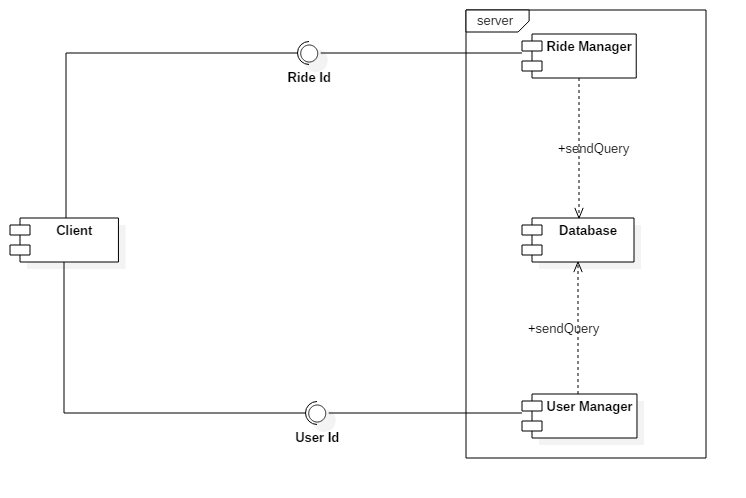
\includegraphics[width=\textwidth]{high_lvl_comp.png}
	\end{figure}
	\newpage
	
\subsection{Component view}
	Here we will provide a more detailed description of the components presented in the previous section.
	\subsubsection{Client component}
	The client is composed by a main component which will have all the basics functions: create account, make request, make reservation; a user interface component that will serve to communicate with the user and finally a connection component that will take care of communicating with the server.
		\begin{figure}[h!]
			\centering
			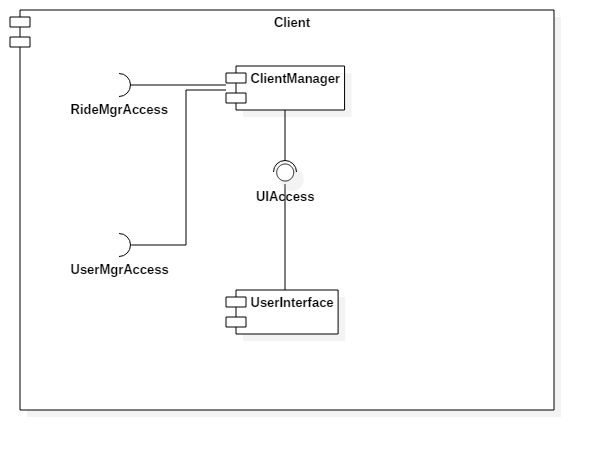
\includegraphics[width=\textwidth]{client.png}
		\end{figure}
		\newpage

	\subsubsection{Ride manager component}
		The ride manager will have a request handler that will take requests or reservation from passengers and forward it to taxi drivers, once a driver has accepted it the ride will be created through the ride generator component. The taxi will be found using the taxi queues manager component. There will be also a connection manager component and a database access component used to access the database.
		\begin{figure}[h!]
			\centering
			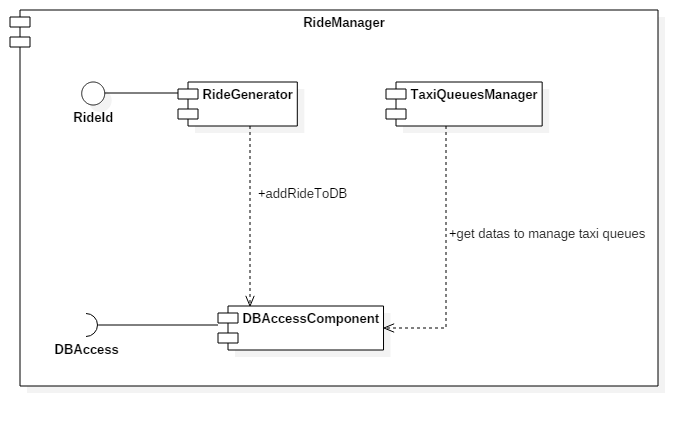
\includegraphics[width=\textwidth]{ride_mgr.png}
		\end{figure}
		\newpage

	\subsubsection{User manager component}
		The user manager will have a account manager component which will provide login and registration functionalities, an account creator component to create new accounts and a database access component.
		\begin{figure}[h!]
			\centering
			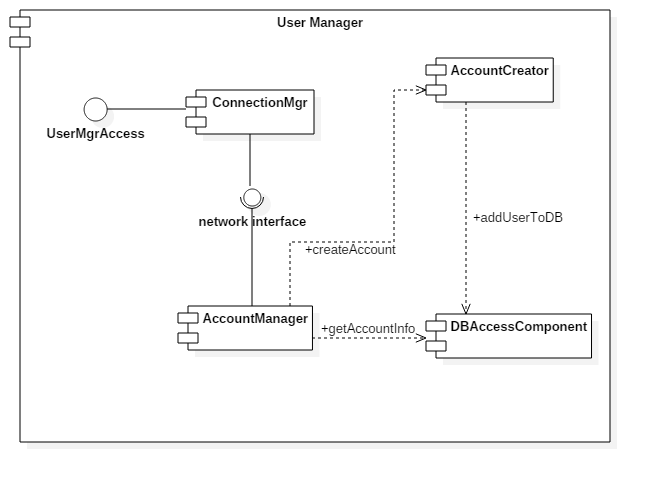
\includegraphics[width=\textwidth]{user_mgr.png}
		\end{figure}
		\newpage
	
	\subsubsection{Database}
	\begin{figure}[h!]
		\centering
%		\includegraphics[width=\textwidth]{ER.png}
	\end{figure}
	\newpage		

\subsection{Deployment view}
This diagram shows how the whole system will be deployed.
A four tier application, with the client, the web server which is responsible to generate web pages and will contain also user manager component, the application server which contains all the taxi management application's logic and the database.
Client, web server and application server communicate with each other through RMI, while the application server uses JDBC to access the database.
	\begin{figure}[h!]
		\centering
		\includegraphics[width=\textwidth]{deployment.png}
	\end{figure}
	\newpage

\subsection{Runtime view}
%sequence diagram tra componenti

\subsection{Component interfaces}

\subsection{Selected architectural styles and patterns}
%credo mvc e cose

\subsection{Other design decisions}